\subsection{Union, Intersection, Difference, and Complement}

\begin{remark} \label{rem:set-builder-notation} \hlt{Set-Builder Notation}\\
$\{x\in X:P(x)\}$ means all $x\in X$ satisfying $P(x)$.\\
For sets $(A_n)$, $\bigcup_nA_n$ means membership in some $A_n$; $\bigcap_nA_n$, membership in every $A_n$.\\
\hlt{Key Insight}: Expand membership conditions.
\end{remark}

\begin{proposition} \label{prop:analysis-set-algebra} \hlt{Basic Set Algebra}\\
Let $A,B,C\subseteq X$. Then
\begin{enumerate}[label=(\roman*)]
\setlength{\itemsep}{0pt}
\item $A\cap(B\cup C)=(A\cap B)\cup(A\cap C)$;
\item $A\cup(B\cap C)=(A\cup B)\cap(A\cup C)$;
\item $(A\cup B)^c=A^c\cap B^c$;
\item $(A\cap B)^c=A^c\cup B^c$.
\end{enumerate}
\begin{proof}
It suffices to prove (i) and (iii); the others are similar. Let $x\in X$. Then
\begin{enumerate}[label=(\roman*)]
\setlength{\itemsep}{0pt}
\item[(i)] $x\in A\cap(B\cup C) \Longleftrightarrow x\in A \text{ and } (x\in B \text{ or } x\in C) \Longleftrightarrow (x\in A\cap B) \text{ or } (x\in A\cap C) \Longleftrightarrow x\in (A\cap B)\cup(A\cap C)$
\item[(iii)] $x\in (A\cup B)^c \Longleftrightarrow x\notin A\cup B \Longleftrightarrow x\notin A \text{ and } x\notin B \Longleftrightarrow x\in A^c\cap B^c$
\end{enumerate}
\hlt{Structural Commentary}: Set algebra is membership logic.\\
\hlt{Key Insight}: Translate sets into conditions on $x$.
\end{proof}
\end{proposition}

\begin{figure}[H]
    \centering
    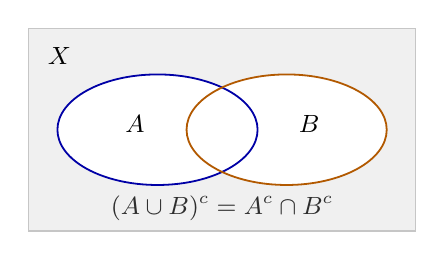
\begin{tikzpicture}[
  x=0.82cm,
  y=0.78cm,
  every node/.style={font=\small},
  ambient/.style={draw=gray!45, fill=gray!12, line width=0.5pt},
  setA/.style={draw=blue!65!black, line width=0.65pt},
  setB/.style={draw=orange!70!black, line width=0.65pt}
]
  \draw[ambient] (-3,-1.65) rectangle (3,1.65);
  \fill[white] (-1.0,0) ellipse (1.55 and 0.9);
  \fill[white] (1.0,0) ellipse (1.55 and 0.9);
  \draw[setA] (-1.0,0) ellipse (1.55 and 0.9);
  \draw[setB] (1.0,0) ellipse (1.55 and 0.9);

  \node at (-1.35,0.1) {$A$};
  \node at (1.35,0.1) {$B$};
  \node[anchor=north west] at (-2.85,1.5) {$X$};
  \node[gray!35!black] at (0,-1.28) {$(A\cup B)^c=A^c\cap B^c$};
\end{tikzpicture}

    \caption{De Morgan's law says that being outside a union is the same as being outside each set.}
    \label{fig:de-morgan-complement-union}
\end{figure}

\begin{theorem} \label{thm:metric-de-morgan-laws} \hlt{Arbitrary De Morgan Laws}\\
Let $X$ be a set. For any collection $\{E_\alpha\}$ of subsets of $X$, $\left(\bigcup\limits_\alpha E_\alpha\right)^c=\bigcap\limits_\alpha E_\alpha^c$ and $\left(\bigcap\limits_\alpha E_\alpha\right)^c=\bigcup\limits_\alpha E_\alpha^c$.
\begin{proof}
The first identity follows from membership: $x\in\left(\bigcup\limits_\alpha E_\alpha\right)^c$ $\Longleftrightarrow$ $x\notin E_\alpha \ \forall \alpha$ $\Longleftrightarrow$ $x\in\bigcap\limits_\alpha E_\alpha^c$.\\
The second follows by applying the first identity to the complements $E_\alpha^c$, or by the same membership argument.\\
\hlt{Structural Commentary}: Complements exchange unions and intersections.\\
\hlt{Key Insight}: Negating ``for some'' gives ``for every'', and conversely.
\end{proof}
\end{theorem}
